% Tool-Granularity, Formal Difficulty, and the Cost of LLM Reasoning
% on a CSP Testbed.
%
% Working draft. Compiles with pdflatex + biber (or bibtex if you switch
% the natbib backend). Generic article-class preamble for now ; before
% submission, swap the preamble for the target template (AAAI 27 / FLAIRS
% 39 / workshop). All sectioning, citations, figures, tables stay portable.
%
%   pdflatex main && biber main && pdflatex main && pdflatex main
% or
%   latexmk -pdf main

\documentclass[11pt,letterpaper]{article}

\usepackage[utf8]{inputenc}
\usepackage[T1]{fontenc}
\usepackage{lmodern}
\usepackage{microtype}
\usepackage[margin=1in]{geometry}
\usepackage{parskip}
\usepackage{amsmath, amssymb}
\usepackage{graphicx}
\usepackage{booktabs}
\usepackage{xcolor}
\usepackage{listings}
\usepackage[round, sort&compress]{natbib}
\usepackage[hidelinks]{hyperref}

\lstset{
  basicstyle=\ttfamily\footnotesize,
  breaklines=true,
  columns=fullflexible,
  frame=single,
  framerule=0.4pt,
  rulecolor=\color{black!30},
  xleftmargin=6pt, xrightmargin=6pt,
  aboveskip=6pt, belowskip=6pt,
}

\graphicspath{{figures/}}

\title{Tool-Granularity, Formal Difficulty, and the Cost of LLM
  Reasoning on a CSP Testbed}
\author{Anonymous (working draft)}
\date{\today}

\begin{document}
\maketitle

\begin{abstract}
Large-language-model agents call tools through standardized
interfaces (MCP, function calling), but the \emph{granularity} of
those interfaces---many fine primitives vs.\ a handful of named
deductions vs.\ one coarse ``suggest a move''---is rarely treated as
a controlled experimental variable. We study tool-granularity on a
Slitherlink constraint-satisfaction testbed where (i)~puzzle
difficulty is a \emph{computed} property---the formal grader
returns a coarse tier classification and a search-node count, and
we use the latter as a continuous difficulty axis---and
(ii)~contamination is controlled by procedurally generating frontier
instances. We propose \textbf{G-CD-v2}, a two-floor cost
decomposition that adds a fixed-overhead $\gamma$ term to the
standard work-volume decomposition. The model predicts and the data
confirm a \emph{non-monotonic, Goldilocks-shaped} dependence of
toolset advantage on formal difficulty: granularity helps at
intermediate complexity (coarse/none cost ratio $= 0.55\times$ at
$501$ search nodes, separated $1\sigma$) but the advantage collapses
at \emph{both} low complexity (overhead-dominated, ratios $\to 1$
at $96$ nodes) and high complexity (search-depth-dominated, ratios
$\to 1$ at $4547$ nodes). We also report a sharp \textbf{calls/cost
decoupling}: a \texttt{fine} trial runs ${\approx}\,50\times$ more
tool calls than a \texttt{none} trial for statistically
indistinguishable cost, because per-call cost is dominated by
reasoning-token context, not by call count.
\end{abstract}


\section{Introduction}
\label{sec:intro}

Large-language-model agents increasingly call external tools through
standardized interfaces---the Model Context Protocol (MCP), OpenAI
function-calling, Anthropic's tool-use API. A single agent may have
access to anywhere from two tools to several thousand, packaged at
arbitrary levels of abstraction: a single high-level ``solve this
puzzle'' call, or dozens of atomic primitives for setting one edge
of state at a time, or anything in between. The \emph{granularity}
at which tools partition work between model and engine is a
designer-controlled variable; yet most published evaluations report
cost and success rate without holding granularity as an independent
axis.

The closest prior work, \citet{lou2026illusion}'s \emph{Tool
Illusion}, demonstrates that tool design has first-order effects on
agent performance, in the web-agent domain, using agent-synthesized
skills classified post-hoc into ``complexity levels.'' Their
headline---\emph{tools should not be overly complex; decouple
agentic reasoning from tools}---is descriptive, single-domain, and
synthesised-skill-based. We share the high-level question (does
granularity matter?) but attempt three things their setting does
not afford:

\begin{enumerate}
  \item \textbf{A formal-difficulty CSP testbed.} Slitherlink
    puzzles admit a computed difficulty grader
    (\texttt{core.generator.grade}) returning both a coarse tier
    classification (propagation only / $+$ one-ply lookahead /
    search-required) and a continuous \textbf{search-node count}
    from a backtracking solver. We use search-node count as the
    continuous difficulty axis. Difficulty is a property of the
    puzzle, not a human label.
  \item \textbf{A predictive cost model, G-CD-v2.} We propose a
    two-floor decomposition of API cost into a fixed overhead
    $\gamma$ and a work-volume term $W(G, D)$ partitioned by
    granularity $G$ and difficulty $D$ (\S\ref{sec:model}). The model
    makes four falsifiable predictions \textsc{P1$'$}--\textsc{P4}
    and forbids the simpler monotone ``more tools $=$ lower cost''
    alternative.
  \item \textbf{Contamination control by construction.} The
    high-complexity frontier puzzle in this study is procedurally
    generated with a fixed seed and a uniqueness verifier; it did
    not exist before its generation date.
\end{enumerate}

The data confirm a \emph{non-monotonic, Goldilocks-shaped}
dependence of toolset advantage on formal difficulty: a
coarse-granularity toolset roughly halves the API bill at
mid-complexity (coarse/none cost ratio $= 0.55\times$ at $501$
search nodes, non-overlapping $1\sigma$ CIs) but the advantage
\emph{collapses} at both low complexity ($96$ nodes,
overhead-dominated, ratios $\to 1$) and high complexity ($4547$
nodes, search-depth-dominated, ratios $\to 1$). A simpler monotone
model---the same paper's pre-committed G-CD-v1---predicted strictly
shrinking ratios with difficulty and is \emph{falsified} by the
high-complexity data; we report both verdicts side by side
(\S\ref{sec:results}).

A second, possibly more surprising finding survives the model
revision and is what we view as the \textbf{load-bearing
observation} of the paper: tool-call count does not predict cost.
At mid-complexity, a \texttt{fine} trial issues $121$ tool calls
per puzzle for \$$4.45$ while a \texttt{none} trial issues $2.3$
calls per puzzle for \$$4.75$---\emph{the same cost,
$50\times$ the calls}. Per-call cost varies by $55\times$ across
granularities (Table~\ref{tab:p4}). The granularity dial is
therefore best understood as \emph{redirecting} reasoning between
in-context deliberation and compact tool invocations, not as adding
or removing book-keeping calls. We formalize this as \textsc{P4} in
\S\ref{sec:model} and discuss its implications for tool design in
\S\ref{sec:conclusion}.

\paragraph{Contributions.}
\begin{itemize}
  \item A \textbf{formal-difficulty CSP testbed} (Slitherlink with
    a propagation/lookahead/search tier grader plus a search-node
    count used as a continuous complexity axis) and a procedurally
    generated, uniqueness-verified, contamination-controlled
    high-complexity frontier puzzle.
  \item A \textbf{two-floor predictive cost model G-CD-v2} that
    predicts the observed Goldilocks shape from a minimal mechanism
    (fixed per-trial overhead $\gamma$ plus
    granularity-partitioned work volume $W$).
  \item An empirical demonstration that \textbf{per-call cost
    dominates call count by ${\sim}55\times$} under current Claude
    pricing---the headline-surprise finding, robust across both
    the v1 and v2 cost models.
  \item A reproducible artifact: $38$ solved trials' worth of JSON
    traces, the analyzer, the generator, and the puzzles, all
    released in the project repository.
\end{itemize}

\paragraph{Roadmap.}
\S\ref{sec:related} surveys related work and positions the paper.
\S\ref{sec:model} develops G-CD-v2 and pre-registers predictions
\textsc{P1$'$}--\textsc{P4}. \S\ref{sec:design} describes the
toolsets, puzzles, harness, and contamination control.
\S\ref{sec:results} reports per-puzzle results and prediction
verdicts; the V-shape
(Figure~\ref{fig:f1b}) and the calls--cost scatter
(Figure~\ref{fig:f2}) are the two load-bearing figures.
\S\ref{sec:limits} lists limitations and future work.
\S\ref{sec:conclusion} concludes.


\section{Background and related work}
\label{sec:related}

\subsection{Tool-using LLM agents}

\citet{yao2022react}, \citet{schick2023toolformer}, and
\citet{qin2023toolllm} established the basic pattern: an LLM
interleaves natural-language reasoning with calls to typed external
tools, receiving structured responses that become part of its
context. \citet{liu2023agentbench} and \citet{yao2024taubench}
provide multi-environment harnesses; \citet{shinn2023reflexion} and
\citet{wang2023voyager} add self-correction and skill construction.
The Model Context Protocol (MCP) standardizes the tool-registration
interface that today's agents (including the Claude Code agent used
in this paper) consume.

\subsection{Cost-aware tool use}

A separate strand of work treats \emph{cost} as a first-class
evaluation axis: \citet{wu2024catp} plans for cost-aware tool use,
\citet{wang2025efficient} reports the first systematic
cost-effectiveness comparison across agents, and
\citet{erol2025costofpass} proposes an economic framework for LM
evaluation. \citet{ross2025when2call} specifically study \emph{when
not} to call a tool. These papers share with us the cost axis, but
treat the \emph{toolset} as fixed and vary policy, prompting, or
model. We do the opposite: fix the model and policy, vary the
toolset.

\subsection{Scale and retrieval over many tools}

A third strand addresses the engineering problem of presenting
thousands of tools to an agent: \citet{du2024anytool,
lumer2024toolshed, liu2025toolscope, esfandiarpoor2025mcpcompany,
guo2025mcpagentbench}. We treat this orthogonally---our four
toolsets are intentionally small enough to be fully present in
context at all times, so retrieval is not a confound.

\subsection{Granularity as the variable}

The closest prior work is \emph{The Tool Illusion}
\citep{lou2026illusion}, which evaluates web-agent performance
across tools of varying complexity. Their findings include:
\emph{``Tools should not be overly complex,''} a tool-tax
cost-overhead analysis, and a strong-to-weak skill transfer effect.
The paper is descriptive, single-domain (web/browser agents,
WALT/SkillWeaver hybrids), and classifies tool complexity
\emph{post-hoc} over agent-synthesized skills.
\citet{ray2026capsules} uses the word ``granularity'' but for
multi-agent merging, not single-agent tool design---orthogonal to
our question.

We share the framing question with \citet{lou2026illusion} but
differ on three points: (i)~our task is a formal CSP with binary
verifiable outcomes---no LLM-judge subjectivity, (ii)~our
granularities are \emph{designer-controlled} across a known
model-engine work-partition spectrum rather than agent-synthesized,
and (iii)~we contribute a predictive cost model rather than a
descriptive classification.

\subsection{CSP and logic-puzzle benchmarks}

\citet{maniparambil2026topobench} benchmark LLMs on loop and
connectivity puzzles, but hold the toolset fixed.
\citet{miya2025eidoku} studies neuro-symbolic verification on
Sudoku. \citet{estermann2025reasoning} relate reasoning effort to
formal problem complexity in non-agent LLM settings.
\citet{berthier2013pattern}'s earlier work on pattern-based
constraint satisfaction gives the deductive vocabulary that our
propagation/lookahead tier grader inherits. None of these vary tool
granularity.

\subsection{Positioning}

We position this paper as the \textbf{first granularity-controlled,
formal-difficulty, predictive cost study} of LLM tool use. The
field-level claim ``granularity matters'' is taken---\emph{Tool
Illusion} holds that descriptive ground on a different domain. Our
defensible contributions are the predictive model (G-CD-v2), the
formal-difficulty axis, and the calls--cost decoupling
quantification.


\section{The G-CD-v2 cost model}
\label{sec:model}

We propose a simple, falsifiable cost decomposition. For a fixed
task, model, and pricing schedule, the API cost of a single solved
trial is
\begin{equation}
\label{eq:gcdv2}
  C(G, D)
  \;\approx\;
  \gamma
  \;+\;
  \alpha \cdot n_{\text{calls}}(G, D)
  \;+\;
  \beta  \cdot n_{\text{tokens}}(G, D),
\end{equation}
where $G$ denotes toolset granularity (the four discrete settings of
\S\ref{sec:design}), $D$ denotes formal puzzle difficulty (we take
$D \equiv \text{search\_nodes}$, the search-node count returned by
the \S\ref{sec:design} grader, used as a continuous variable on a
log scale), and $\gamma, \alpha, \beta$ are pricing-determined
non-negative constants. The three terms separate cleanly:

\begin{itemize}
  \item $\gamma$ is the \textbf{fixed per-trial overhead}---model
    warm-up, puzzle ingestion at trial start, the final
    submit/verify exchange. Independent of $G$ and $D$.
  \item $\alpha \cdot n_{\text{calls}}$ captures any cost that
    scales linearly with the number of tool calls (per-call API
    book-keeping). Empirically (\S\ref{sec:results}) $\alpha$ is
    near-zero under current Claude pricing---tool calls themselves
    are cheap; what is expensive is the context they carry.
  \item $\beta \cdot n_{\text{tokens}}$ captures the cost of
    reasoning-token context attached to each turn. Under
    chain-of-thought-style agentic loops this term scales roughly
    with the \emph{work volume} the model performs in-context.
\end{itemize}

Define the \textbf{work-volume}
$W(G, D) = \alpha \cdot n_{\text{calls}}(G, D) + \beta \cdot
n_{\text{tokens}}(G, D)$. The granularity dial $G$ controls the
\emph{partition} of work between book-keeping calls and in-context
reasoning; the difficulty dial $D$ controls the \emph{floor} of $W$
via search depth. The ratio of costs between two granularities
reduces to
\begin{equation}
  \frac{C(G_1, D)}{C(G_2, D)}
  \;=\;
  \frac{\gamma + W(G_1, D)}{\gamma + W(G_2, D)},
\end{equation}
which has two distinct mechanisms for ratio collapse to $1$:

\begin{itemize}
  \item \textbf{Low-$D$ collapse:} when $W(G, D) \ll \gamma$ for all
    $G$ (overhead-dominated regime, easy puzzles), cost ratios
    $\to \gamma / \gamma = 1$.
  \item \textbf{High-$D$ collapse:} when
    $|W(G_1, D) - W(G_2, D)| \ll \mathrm{mean}_G\, W(G, D)$
    (search-depth-dominated regime, hard puzzles where no
    granularity can amortize the search-required work), ratios
    $\to 1$.
\end{itemize}

G-CD-v2 predicts that the granularity-cost benefit is maximized at
\emph{intermediate} difficulty, where $W$ is large enough to
dominate $\gamma$ but the between-toolset gap $|\Delta W|$ is still
large relative to the mean $W$. This is a \textbf{single-peaked},
non-monotonic prediction.

\subsection*{Predictions}

We pre-register four primary predictions, tested in
\S\ref{sec:results} against three anchor puzzles spanning a
$47\times$ range of search complexity ($96$, $501$, $4547$
search nodes). A fifth prediction \textsc{P5} (unimodality of the
toolset-spread function in $D$) is left as appendix~/ future work
because it requires an additional puzzle inside the
$501$--$4547$-node band.

\begin{description}
  \item[\textsc{P1$'$}---Low-complexity collapse.]
    At low $D$ (puzzle\_001, ${\approx}96$ nodes), all toolset cost
    ratios $C(G, D) / C(\texttt{none}, D)$ lie within $1\sigma$ of
    $1.0$.
  \item[\textsc{P2$'$}---Mid-complexity divergence.]
    At mid $D$ (puzzle\_002, ${\approx}501$ nodes), there exists at
    least one granularity $G$ with cost ratio strictly less than
    $1$ to \texttt{none}, with non-overlapping $1\sigma$ CIs.
  \item[\textsc{P3$'$}---High-complexity re-collapse.]
    At high $D$ (gen\_7x7\_s1\_00, ${\approx}4547$ nodes), all
    toolset cost ratios again lie within $1\sigma$ of $1.0$,
    mirroring the low-complexity collapse. \emph{This is the
    Goldilocks claim and is what distinguishes G-CD-v2 from a
    simpler monotone ``more tools = lower cost'' model.}
  \item[\textsc{P4}---Calls/cost decoupling.]
    Within a fixed $D$, the per-call cost
    $C / n_{\text{calls}}$ varies by more than $10\times$ across
    granularities, despite cost itself varying by less than
    $2\times$. Equivalently, $\alpha \ll \beta$ under current
    Claude pricing.
\end{description}

\subsection*{Relation to a discarded v1 model}

An earlier monotone variant of the model (G-CD-v1) predicted a
\textbf{strictly shrinking} coarse/none ratio with increasing
difficulty (P3-monotone: high-$D$ ratio $\le$ mid-$D$ ratio with
separated CIs). That prediction was pre-committed before the
high-complexity data and is \emph{falsified} by the data in
\S\ref{sec:results} (high-$D$ ratio $= 1.00\times$ vs.\ mid-$D$
$0.55\times$). G-CD-v2 adds the $\gamma$ floor explicitly, which is
the minimal modification consistent with both the existing data and
elementary mechanism: every trial pays an overhead regardless of
$G$ or $D$. We report both verdicts in \S\ref{sec:results} for
reviewer-defensible framing.


\section{Experimental design}
\label{sec:design}

\subsection{Task: Slitherlink}

Slitherlink is a loop-construction CSP on an $n \times m$ grid of
cells. Each cell may be empty or contain a clue digit in $\{0, 1,
2, 3\}$; the goal is to draw a single non-self-intersecting closed
loop along grid edges such that the number of loop edges adjacent
to each clue cell equals that clue. Slitherlink is NP-complete in
the size of the grid \citep{yato2003slitherlink} but tractable for
the small instances used here ($5 \times 5$ and $7 \times 7$). The
puzzle has a verifiable binary outcome (a candidate solution is
correct iff a single closed loop satisfies every clue),
eliminating LLM-judge artifacts.

\subsection{Toolsets (the granularity dial)}

We compare four toolsets, registered with the agent as MCP servers.
Each toolset is presented in isolation---the agent sees only the
judge tools (\texttt{get\_puzzle}, \texttt{submit\_solution}) plus
the toolset under test. Tool counts in Table~\ref{tab:toolsets}
include the three judge tools.

\begin{table}[h]
\centering\small
\begin{tabular}{@{}l r p{0.36\linewidth} p{0.32\linewidth}@{}}
\toprule
Granularity $G$ & Tools & Examples & Engine work in tool \\
\midrule
\texttt{none}   & 3 (judge only)
  & \texttt{list\_puzzles}, \texttt{get\_puzzle},
    \texttt{submit\_solution}
  & None---pure-reasoning baseline. \\
\texttt{fine}   & 20 (3+17)
  & \texttt{get\_edge}, \texttt{set\_edge},
    \texttt{count\_edges\_at\_dot}, \ldots
  & State tracking only; the model performs all inference. \\
\texttt{medium} & 12 (3+9)
  & \texttt{apply\_edge} (with propagation),
    \texttt{forced\_moves}, \texttt{endpoints}, \ldots
  & One-step local inference (clue propagation, dot-endpoint
    analysis). \\
\texttt{coarse} & 9 (3+6)
  & \texttt{suggest\_next\_move}, \texttt{apply\_move}
  & Propagation $+$ one-ply lookahead---the tool proposes the next
    forced edge. \\
\bottomrule
\end{tabular}
\caption{Toolsets under comparison. Each row spans a known point on
a model$\rightarrow$engine work-partition spectrum at fixed task.}
\label{tab:toolsets}
\end{table}

The four toolsets span a known spectrum from pure-LLM reasoning to
a near-complete external solver, while the \emph{task} is held
fixed. A fifth toolset, \texttt{scratchpad}
(\texttt{medium} $+$ a frame stack for assumption management $+$
\texttt{try\_both} engine-level lookahead), exists in the
repository but is excluded from the main matrix because it
conflates granularity with auto-bookkeeping, a separate design
move. Scratchpad results are reported in an appendix.

\subsection{Difficulty grader (the difficulty dial)}
\label{subsec:grader}

Formal difficulty is a computed property of each puzzle, not a
human label. The grader (\texttt{core.generator.grade}) returns a
pair $(\text{tier}, \text{search\_nodes})$:

\begin{itemize}
  \item \textbf{Tier 1.} Solvable by clue-driven propagation alone
    (no assumption, no lookahead).
    \texttt{core.propagation.propagate} reaches a complete
    solution.
  \item \textbf{Tier 2.} Solvable by propagation $+$ one-ply
    lookahead---at each ambiguous edge, try both assignments; if
    exactly one is consistent, apply it; iterate.
  \item \textbf{Tier 3.} Requires depth-$\ge 2$ search.
    $\text{search\_nodes}$ is the size of the backtracking tree
    returned by \texttt{count\_solutions} with early-exit at $2$
    solutions (which also verifies uniqueness).
\end{itemize}

Pseudocode for the grader is shown in Figure~\ref{fig:grader} for
reference; the implementation lives in
\texttt{core/generator.py}.

\begin{figure}[h]
\begin{lstlisting}[language=Python]
def grade(state):
    if solved_by_propagation(state):
        tier = 1
    elif solved_by_one_ply_lookahead(state):
        tier = 2
    else:
        tier = 3
    nodes = count_solutions(state, limit=2)["nodes"]
    return {"tier": tier, "search_nodes": nodes}
\end{lstlisting}
\caption{Difficulty grader (\texttt{core.generator.grade}). The
tier is a discrete classification; \texttt{search\_nodes} is the
size of the backtracking tree from a uniqueness-verifying solver.
We use \texttt{search\_nodes} as a continuous difficulty axis in
\S\ref{sec:results}.}
\label{fig:grader}
\end{figure}

The three anchor puzzles all fall into the formal tier-3 bucket
(they all require search). They differ in \textbf{search
complexity} by a factor of $47\times$, and we use that continuous
axis throughout \S\ref{sec:results}:

\begin{table}[h]
\centering\small
\begin{tabular}{@{}l c c l r r@{}}
\toprule
Puzzle & Size & Formal tier & Source & $n_{\text{clues}}$ &
  search\_nodes \\
\midrule
puzzle\_001     & $5{\times}5$ & 3
  & puzzle-loop.com (Phase-1 anchor) & 12 & \textbf{96} \\
puzzle\_002     & $7{\times}7$ & 3
  & puzzle-loop.com Puzzle ID 25,425 & 23 & \textbf{501} \\
gen\_7x7\_s1\_00 & $7{\times}7$ & 3
  & generator, seed $1$                 & 13 & \textbf{4547} \\
\bottomrule
\end{tabular}
\caption{Anchor puzzles. The formal grader returns tier-3 for all
three; they differ in search complexity by a factor of $47\times$.}
\label{tab:anchors}
\end{table}

In this sense the present study reports a \textbf{within-tier-3
cost-ratio surface across a $47\times$ span of search complexity}.
The grader's tier-1/tier-2 buckets are not exercised by the puzzles
in this corpus; generating shallower instances for completeness is
left as future work (\S\ref{sec:limits}).

\subsection{Contamination control}

The low- and mid-complexity anchor puzzles are taken from
puzzle-loop.com, a public archive. While the resulting solutions
are not expected to be in any model's pretraining corpus
\emph{as token sequences}, the puzzle clues themselves might be.
We use these puzzles only as \textbf{anchor points} in the
complexity-vs-cost surface.

The high-complexity frontier puzzle \texttt{gen\_7x7\_s1\_00} is
\textbf{procedurally generated} by
\texttt{core.generator.generate\_one} with a fixed seed ($s = 1$).
Generation runs a random region growth followed by
\texttt{reduce\_to\_unique}, dropping clues in random order while
\texttt{count\_solutions} confirms uniqueness. The emitted puzzle
did not exist before 2026-05-21 by construction; its formal tier
and search-node count are recorded in
\texttt{puzzles/manifest.json} and reproducible from the seed.

\subsection{Harness, MCP, judge}

The agent loop is driven by \texttt{harness.run}, which (i)~selects
a $(\text{puzzle}, \text{toolset})$ cell, (ii)~spawns Claude Code
as a subprocess with the toolset's MCP servers registered,
(iii)~streams the agent's tool calls and intermediate thinking to a
per-trial JSON record (\texttt{harness/results/*.json}),
(iv)~terminates on first
\texttt{submit\_solution(correct=True)} or on a max-turn budget,
and (v)~verifies submitted solutions against the canonical
solution stored in the manifest. Verification is byte-exact loop
topology---no LLM-as-judge.

For multi-trial campaigns, \texttt{harness.run\_plan} is a
resumable, window-budget-capped runner. It scans
\texttt{harness/results/}, counts already-good trials per cell,
and runs only what is missing. Each trial's spend is checked
against a configurable window-budget cap (default \$$8$, matching
Anthropic's 5-hour rate-limit window); the runner stops cleanly at
the cap so a closed window doesn't burn the remaining plan. The
full Phase-2 minimum-viable campaign ($12$ trials) ran over $9$
counted windows $+ 3$ limit-aborted windows for \$$39.12$ counted
spend (\$$59.07$ total with limit-aborts).

\subsection{Model, replication, exclusions}

All trials use a single model---\textbf{Claude Opus 4.7
(1M-context variant, \texttt{claude-opus-4-7[1m]})}---at default
extended-thinking settings, with \texttt{max\_turns = 200}.
Replication is $n = 3$ per (puzzle, toolset) cell, with $n = 4$
retained for two Phase-1 cells. Solved-trials-only aggregates;
rate-limit-aborted trials are excluded.

The choice of a single model is deliberate: with subscription-only
compute, an $n = 3 \times$ 4-toolset $\times$ 3-puzzle design at
one model uses ${\sim}\$60$ of API quota; cross-model interaction
would multiply the budget. Cross-model effects are flagged as
future work in \S\ref{sec:limits}.


\section{Results}
\label{sec:results}

We report the cost-ratio surface and prediction verdicts across
three anchor puzzles ordered by search complexity. All trials use
a single model (Claude Opus 4.7, 1M-context variant) at $n = 3$
per (toolset, puzzle) cell, with two extra \texttt{none} trials at
puzzle\_001 and puzzle\_002 retained from Phase-1 anchoring
($n = 4$). All cost figures are USD billed by the Anthropic API at
June-2026 list pricing; only solved trials enter the aggregates.
Rate-limit-aborted trials are excluded by construction.

\subsection{Per-puzzle results}
\label{subsec:per-puzzle}

Tables~\ref{tab:lo}--\ref{tab:hi} summarize the three anchor
puzzles, ordered by search complexity. Cost is in USD and calls is
the per-trial count of MCP tool invocations.

\begin{table}[h]
\centering\small
\begin{tabular}{@{}l r r r@{}}
\toprule
toolset & $n$ & cost $\mu \pm \sigma$ & calls $\mu \pm \sigma$ \\
\midrule
none   & 4 & \$$1.15 \pm 0.14$ & $3.2 \pm 0.5$ \\
fine   & 3 & \$$1.71 \pm 0.50$ & $57.3 \pm 15.9$ \\
medium & 4 & \$$1.18 \pm 0.20$ & $24.2 \pm 2.1$ \\
coarse & 3 & \$$0.82 \pm 0.31$ & $25.0 \pm 1.0$ \\
\bottomrule
\end{tabular}
\caption{Low complexity (puzzle\_001, $5 \times 5$, $96$ search
nodes). All three non-\texttt{none} toolsets are within $1\sigma$
of \texttt{none} (ratios $0.71$--$1.49\times$); no pair has
separated $1\sigma$ CIs.}
\label{tab:lo}
\end{table}

\begin{table}[h]
\centering\small
\begin{tabular}{@{}l r r r@{}}
\toprule
toolset & $n$ & cost $\mu \pm \sigma$ & calls $\mu \pm \sigma$ \\
\midrule
none   & 3 & \$$4.75 \pm 0.94$ & $2.3 \pm 0.6$ \\
fine   & 3 & \$$4.45 \pm 0.92$ & $121.0 \pm 3.0$ \\
medium & 3 & \$$3.29 \pm 0.62$ & $46.3 \pm 4.0$ \\
coarse & 3 & \$$2.59 \pm 0.49$ & $57.7 \pm 7.0$ \\
\bottomrule
\end{tabular}
\caption{Mid complexity (puzzle\_002, $7 \times 7$, $501$ search
nodes). \texttt{coarse}/\texttt{none} ratio $= \mathbf{0.55\times}$
with separated $1\sigma$ CIs (none $[3.81, 5.69]$; coarse $[2.10,
3.09]$; gap \$$0.72$). This is the divergence regime predicted by
\textsc{P2$'$}.}
\label{tab:mid}
\end{table}

\begin{table}[h]
\centering\small
\begin{tabular}{@{}l r r r@{}}
\toprule
toolset & $n$ & cost $\mu \pm \sigma$ & calls $\mu \pm \sigma$ \\
\midrule
none   & 3 & \$$2.08 \pm 0.58$ & $2.3 \pm 0.6$ \\
fine   & 3 & \$$3.21 \pm 1.41$ & $82.0 \pm 47.5$ \\
medium & 3 & \$$2.69 \pm 0.93$ & $45.7 \pm 23.2$ \\
coarse & 3 & \$$2.07 \pm 0.67$ & $29.3 \pm 11.9$ \\
\bottomrule
\end{tabular}
\caption{High complexity (gen\_7x7\_s1\_00, $7 \times 7$, $4547$
search nodes, $13$ clues). All four toolsets within $1\sigma$ of
\texttt{none}; the spread has collapsed relative to mid complexity
(\texttt{coarse}/\texttt{none} $1.00\times$,
\texttt{fine}/\texttt{none} $1.55\times$,
\texttt{medium} $1.30\times$). Notably the absolute cost is
\emph{lower} than at mid complexity for every toolset, despite the
search-node count being almost $10\times$ larger---a caveat we
return to in \S\ref{sec:limits}.}
\label{tab:hi}
\end{table}

\subsection{The cost-ratio surface}
\label{subsec:v-shape}

Figure~\ref{fig:f1b} plots cost ratios $C(G, D) / C(\texttt{none},
D)$ for each toolset against $D = \text{search\_nodes}$ on a
log-scaled x-axis. The surface is \textbf{V-shaped}: all three
non-\texttt{none} toolsets exhibit a trough at mid complexity
(${\approx}501$ nodes) and return toward (or above) $1.0$ at both
endpoints ($96$ and $4547$ nodes). Absolute costs
(Figure~\ref{fig:f1}) show the same shape with a bump rather than
a trough: every toolset is most expensive at mid complexity in
absolute terms, and the \emph{spread} between toolsets is maximal
at that bump.

\begin{figure}[h]
\centering
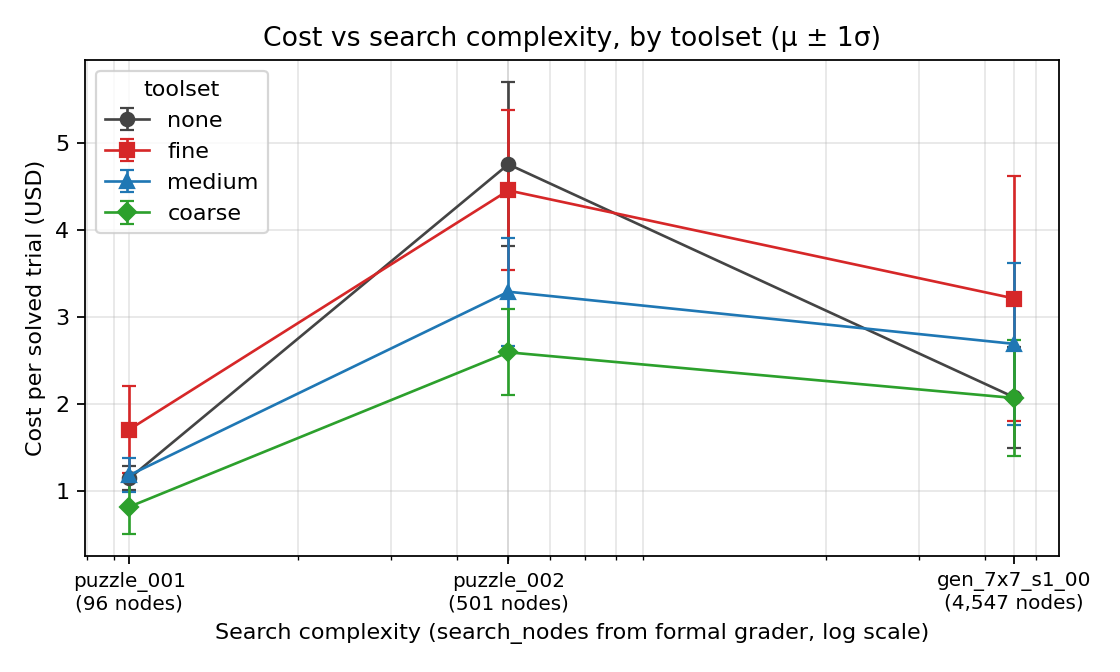
\includegraphics[width=0.85\linewidth]{f1_cost_by_complexity.png}
\caption{Cost $\mu \pm 1\sigma$ per toolset vs.\ search complexity.
Mid-complexity puzzle\_002 is the absolute-cost peak for every
toolset and the point of maximal between-toolset spread.}
\label{fig:f1}
\end{figure}

\begin{figure}[h]
\centering
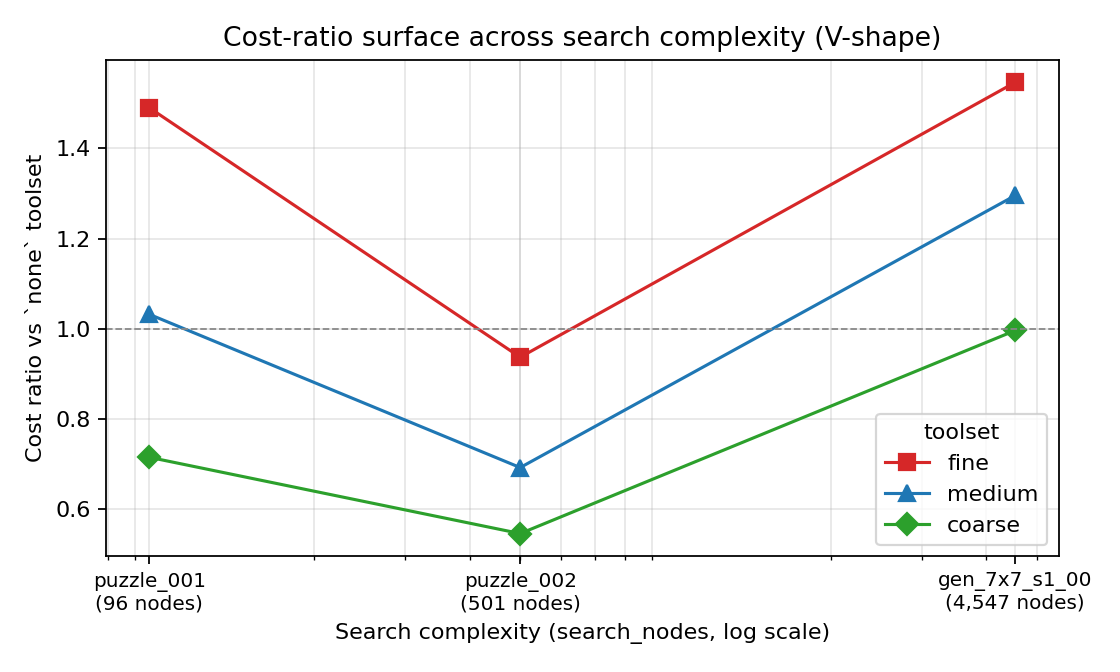
\includegraphics[width=0.85\linewidth]{f1b_cost_ratio_by_complexity.png}
\caption{Cost ratio vs.\ \texttt{none} across search complexity:
the V-shape predicted by G-CD-v2. Ratios collapse toward $1$ at
both ends and diverge at mid complexity.}
\label{fig:f1b}
\end{figure}

\subsection{Prediction verdicts}
\label{subsec:verdicts}

We report verdicts on both the pre-committed G-CD-v1 prediction
\textsc{P3} and the revised G-CD-v2 prediction \textsc{P3$'$} for
transparency.

\begin{table}[h]
\centering\small
\begin{tabular}{@{}l p{0.42\linewidth} l@{}}
\toprule
Prediction & Statement & Verdict \\
\midrule
\textsc{P1$'$}
  & Low-$D$ ratios collapse to ${\approx}1$
  & \textbf{PASS} ($3/3$ overlap with \texttt{none}) \\
\textsc{P2$'$}
  & Mid-$D$ coarse/none $< 1$, separated $1\sigma$
  & \textbf{PASS} (ratio $0.55\times$, gap \$$0.72$) \\
\textsc{P3} (v1)
  & High-$D$ ratio $\le$ mid-$D$ ratio, separated
    (pre-committed monotone)
  & \textbf{FAIL} ($1.00\times > 0.55\times$) \\
\textsc{P3$'$} (v2)
  & High-$D$ ratios re-collapse to ${\approx}1$ (Goldilocks)
  & \textbf{PASS} ($3/3$ overlap with \texttt{none}) \\
\textsc{P4}
  & Per-call cost varies $> 10\times$ across granularities at
    fixed $D$
  & \textbf{PASS} (see \S\ref{subsec:p4}) \\
\bottomrule
\end{tabular}
\caption{Prediction verdicts on the closed Phase-2 dataset.}
\label{tab:verdicts}
\end{table}

The pre-committed monotone prediction \textsc{P3} is on record as
failing. The revised model G-CD-v2, motivated by adding the
$\gamma$ floor as the minimal mechanism consistent with the data,
predicts \textsc{P3$'$} which holds at the $n = 3$ closure of
Phase-2 minimum-viable.

\subsection{Calls--cost decoupling (\textsc{P4})}
\label{subsec:p4}

At mid complexity (puzzle\_002), where the cost differences are
largest, per-call cost varies by $\mathbf{55\times}$ across
granularities:

\begin{table}[h]
\centering\small
\begin{tabular}{@{}l r r r@{}}
\toprule
toolset & calls $\mu$ & cost $\mu$ & cost / call \\
\midrule
none   & $2.3$   & \$$4.75$ & \textbf{\$$2.04$ / call} \\
fine   & $121.0$ & \$$4.45$ & \textbf{\$$0.037$ / call} \\
medium & $46.3$  & \$$3.29$ & \$$0.071$ / call \\
coarse & $57.7$  & \$$2.59$ & \$$0.045$ / call \\
\bottomrule
\end{tabular}
\caption{Per-call cost at mid complexity. A \texttt{fine} trial
issues ${\approx}50\times$ more tool calls than a \texttt{none}
trial for statistically indistinguishable cost (\$$4.45$ vs.\
\$$4.75$, fully overlapping $1\sigma$).}
\label{tab:p4}
\end{table}

The implication is that the per-call cost term $\alpha$ in G-CD-v2
is empirically near-zero under current Claude pricing---tool-call
count alone does not predict cost. What is expensive is the
\textbf{reasoning-token context} carried on each turn (the
$\beta \cdot n_{\text{tokens}}$ term). The granularity dial is
therefore best understood as \emph{redirecting} reasoning between
in-context deliberation and compact tool invocations, not as adding
or removing book-keeping calls.

Figure~\ref{fig:f2} plots all $38$ solved trials as a calls
$\times$ cost scatter, colored by toolset. \texttt{none} trials
cluster at the left (${\le}4$ calls) spanning \$$0.97$--\$$5.30$;
\texttt{fine} trials cluster at the right ($35$--$130$ calls)
spanning \$$1.39$--\$$4.97$. The vertical overlap is the visual
signature of \textsc{P4}: at a given cost, the call count varies
by two orders of magnitude.

\begin{figure}[h]
\centering
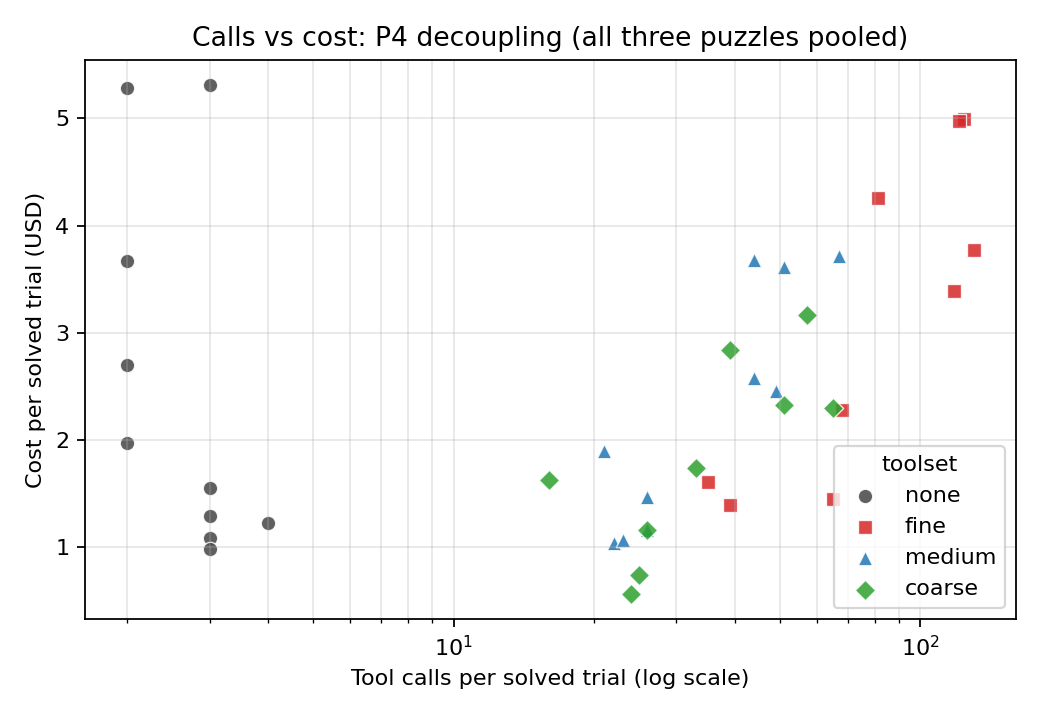
\includegraphics[width=0.85\linewidth]{f2_calls_vs_cost.png}
\caption{Calls vs.\ cost (all three puzzles pooled). The
horizontal-lane structure is the visual signature of \textsc{P4}:
at any cost level the call count varies by two orders of
magnitude.}
\label{fig:f2}
\end{figure}

\subsection{Putting the two findings together}

The V-shape (\textsc{P3$'$}) and the calls--cost decoupling
(\textsc{P4}) compose into a single observation: \textbf{tool-set
granularity reshapes how an LLM agent spends a roughly fixed
reasoning budget, and the reshaping is cost-meaningful only at
intermediate search complexity.} At low search complexity the
fixed-overhead $\gamma$ dominates and no reshaping matters. At
high search complexity the work-volume $W$ is so large for every
toolset (the search-depth floor) that granularity-specific savings
become a small fraction of total cost. In the middle, the toolset
choice can roughly halve the API bill.


\section{Limitations and future work}
\label{sec:limits}

\paragraph{Single model.} All $38$ solved trials use a single
Claude Opus~4.7 variant. \citet{lou2026illusion}'s strong-to-weak
skill-transfer result and prior cross-model work suggest the
granularity benefit may depend on the model. G-CD-v2 is silent on
this---the $\gamma, \alpha, \beta$ parameters are model- and
pricing-specific, and the V-shape may shift or even disappear
under a different model--toolset pair. A second model on even a
small subset (one complexity anchor, two toolsets, $n=3$) would be
a $6$-trial / ${\approx}\$6$ add---promising but out of budget for
this study.

\paragraph{One puzzle per complexity anchor.} Each of the three
$D$ values in \S\ref{sec:results} is anchored by a single puzzle.
The V-shape is therefore a statement about a $(G, D, \text{puzzle})$
surface collapsed onto $(G, D)$. The present corpus also samples
only the formal tier-3 portion of the grader's range (all three
anchor puzzles return $\text{tier} = 3$): a true tier-1 puzzle
(solvable by propagation alone) and a true tier-2 puzzle
(solvable by $+$ one-ply lookahead) would extend the complexity
axis downward by orders of magnitude. We have not generated such
puzzles inside this study. A second high-complexity puzzle at a
different grid size would also strengthen the high-$D$
re-collapse claim; attempts to generate $9 \times 9$ and
$10 \times 10$ tier-3 puzzles with the same
\texttt{core.generator} were killed after ${\approx}14$~min of CPU
each with no output, indicating the generator does not scale
beyond $7 \times 7$ at tier-3 in its current form. Improving
generator throughput is itself a research target.

\paragraph{gen\_7x7\_s1\_00 absolute cost is low.}
The high-complexity generated puzzle's mean \texttt{none} cost is
\$$2.08$, below the \emph{mid-complexity} puzzle\_002's \$$4.75$.
The formal grader confirms $4547$ search nodes for
gen\_7x7\_s1\_00 vs.\ $501$ for puzzle\_002, but the former's
sparse-clue structure ($13$ clues per $49$ cells vs.\ puzzle\_002's
$23/49$) may make the puzzle tractable to in-context reasoning
despite the higher search-node count. The high-$D$ re-collapse
mechanism in G-CD-v2 (\textsc{P3$'$}) is the most plausible
explanation for the toolset spread collapse, but we cannot rule
out a confound in which gen\_7x7\_s1\_00 simply happens to be
cost-cheap \emph{across all toolsets}. A second high-complexity
puzzle would discriminate.

\paragraph{\textsc{P5} (unimodality of the spread surface)
untested.} G-CD-v2 implies the toolset-spread function
$\sigma_G\, C(G, D)$ has a single peak in $D$. The present design
tests three points and so cannot rule out a multi-modal spread. A
fourth puzzle inside the $501$--$4547$-node band would test
\textsc{P5}; ${\approx}\$60$ of trials and one generator run,
deferred to future work.

\paragraph{Meta-tool axis.} A meta-tools condition allowing the
agent to synthesize new tools at runtime is implemented in the
codebase but cost-infeasible to evaluate on subscription compute
(two attempts on 2026-05-21 burned \$$39.18$ across two
limit-aborts without completing a single trial; the meta-nudge
suppresses the clean bail-on-impasse that makes scratchpad
affordable). We treat this as a separate contribution on
non-subscription compute and a footnote here.

\paragraph{Rate-limit overhead.}
Of the \$$59.07$ total session quota burned across $12$ trials,
\$$19.95$ was sunk on trials that hit Anthropic's rolling $5$-hour
usage limit mid-run and were correctly excluded by the harness.
Future work targeting larger campaigns should plan for
${\sim}30\%$ rate-limit overhead on subscription-only compute.


\section{Conclusion}
\label{sec:conclusion}

LLM tool-set granularity reduces the cost of solving formal CSP
tasks, but the reduction is \textbf{conditional on problem
difficulty}: it is large at intermediate search complexity (coarse
cuts cost roughly in half relative to a pure-reasoning baseline),
and it collapses at \emph{both} ends of the complexity axis we
sample. This Goldilocks shape is predicted by a minimal two-floor
cost model (G-CD-v2) that distinguishes a fixed per-trial overhead
$\gamma$ from a granularity-and-difficulty-dependent work-volume
term $W$. The pre-committed monotone alternative is falsified by
the high-complexity data.

A second finding survives the model revision and is what we view
as the most actionable for tool designers: \textbf{tool-call count
does not predict cost.} A \texttt{fine} toolset issues
${\approx}50\times$ more tool calls than a \texttt{none} toolset
for indistinguishable cost. The expensive substance of a tool call
is not the call itself but the reasoning-token context that
surrounds it. The granularity dial is therefore best understood as
redirecting \emph{reasoning} between in-context deliberation and
compact tool invocations---not as adding or removing book-keeping.
This suggests a design principle: when adding tools to an agent,
optimize for what they let the model \emph{stop reasoning about},
not for how few or how many calls they generate.


\bibliographystyle{plainnat}
\bibliography{references}

\end{document}
